\documentclass[12pt]{beamer}
\usetheme{Singapore}
\usepackage[utf8]{inputenc}
\usepackage{amsmath}
\usepackage{amsfonts}
\usepackage{amssymb}
\usepackage{graphicx}


\author{{\textbf{Mohimenul Karim}} \newline And \newline {\textbf{Ankur Lahiry}}}
\title{Huffman Coding}
%\setbeamercovered{transparent} 
%\setbeamertemplate{navigation symbols}{} 
%\logo{} 
%\institute{} 
%\date{} 
%\subject{} 
\begin{document}
	
\begin{figure}

\includegraphics[scale=1.1]{images}
\end{figure}


\begin{frame}
\titlepage
\end{frame}

%\begin{frame}
%\tableofcontents
%\end{frame}
\begin{frame}
		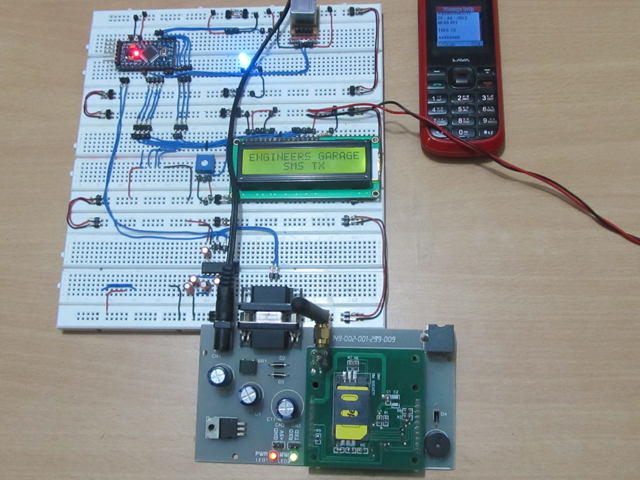
\includegraphics[scale=0.4]{Circuit}
\end{frame}



\begin{frame}
		
\includegraphics[scale=0.6]{error}
\end{frame}

\begin{frame}


			\begin{block} {\color{blue}\textit{{{How To Solve This Problem???}}}} 
			\end{block}
            
            \pause
          
           \begin{block} {\color{orange}\textit{Can we minimize the number of bits for representing the character?} }
			\end{block}           
           
            \pause
           
			\begin{block}          
          		{\color{blue}\textbf{\textit{Yes}}}
          	\end{block}
            
            \pause
			
			\begin{block}          
          		{\color{black}{\textbf{How.........???}}}
          	\end{block}            
            
            \pause
            \begin{block} {We can solve this problem using \color{red}\textbf{\textit{Huffman Coding}}}
          	\end{block}
            
           

\end{frame}
			
\begin{frame}{Principle of Huffman Coding}

\begin{itemize}
	\pause	
	\item {\color{red}\textbf{Huffman Coding}} works in {\color{orange}\textbf{Greedy Approach}}
	\pause
	\item It focuses on {\color{orange}\textbf{frequency}} of each character appearing in the text to construct an optimal binary representation of the characters. 
	
	
\end{itemize}



\end{frame}

\begin{frame} {Greedy Approach}

	\begin{itemize}
		\item Greedy Algorithm always makes the choice that looks best at the moment
	
	\pause
	
	    \item It makes a locally optimal choice for achieving optimal solution 
	
	\pause
	
	     \item Example: `Activity Selection Problem' , `Coin Changing Problem' , `Fractional Knapsack Problem' etc 
	\end{itemize}
	



	
\end{frame}

\begin{frame} {Retriving Lowest Frequency Of Characters}
	
	\pause
	To implement this technique Huffman Algorithm uses Priority Queue 
	\pause
	
	\textbf{\textit{Concepts Of Priority Queue}}
	\begin{itemize}
		\item Is an abstract data type like array where additionally each element has a "priority" associated with it. 
		\item An element with high priority is served before an element with low priority
		\item If two elements have the same priority, they are served according to their order in the queue.
	\end{itemize}
	

	
\end{frame}

\begin{frame} {Back To Huffman Coding}
	\begin{itemize}
		\item Is a procedure to generate a binary code tree 
		\item this was invented by David Huffman in 1952 
	\end{itemize}
 		
 		
\end{frame}


\begin{frame} {Huffman Coding Algorithm}
   \begin{itemize}
   	\item Initializzation: put all symbols on a list sorted according to their frequency counts
    \item Repeat until the list has only one symbol left:\\
		
			a) From the list pick two symbols with the lowest frequency counts\\
   			b) From a Huffman sub-tree that has these two symbols as child nodes and create a parent node\\ 
   			c) Assign the sum of the children's frequency counts to the parent and insert it into the list 					   such that the order is maintained\\
   			d) Delete the children from the list\\
        
   		
   	\item Assign A codeword for each leaf based on the path from the root  
   \end{itemize}
\end{frame}


\begin{frame} {Continued....}
     n = $|$C$|$ \\
     Q = C\\
     \textbf{for} i =1 \textbf{to} n-1:\\
     
     	\qquad 	 allocate a new node z\\
     	\qquad 	 z.left = x= EXTRACT-MIN(Q)\\
     	\qquad 	 z.right = y = EXTRACT-MIN(Q)\\
     	\qquad 	 z.freq = x.freq + y.freq\\
     	\qquad 	 Insert(Q,z)\\
     \textbf{return}  EXTRACT-MIN(Q)
\end{frame}


\begin{frame} {Number of Bits}

	 To encode a file , the total number of bits , B(T) = $ \Sigma c.freq * d_{t}(c) $  \\
	 
	 Where T is the encoded tree\\
	 c belongs to the character set


\end{frame}

\begin{frame} {Back To The MISSISSIPPI RIVER}

	\textit{\textbf{Spliting the word }}

	\pause
     
     \begin{table}[bt]
	\begin{tabular}{|l|c|c|c|c|c|c|c|} \hline 
	\textbf{M} & \textbf{I} & \textbf{S} & \textbf{P} & \textbf{R} & \textbf{V} & \textbf{E} &\textbf{""} \\ \hline
	
	\textbf{1} & \textbf{5} & \textbf{4} & \textbf{2} & \textbf{2} & \textbf{1} & \textbf{1} &\textbf{1} \\ \hline
	\end{tabular}
\end{table}	
	
     
	\pause
	
	\textit{\textbf{Decending Order of Numbers}}
	 
     \begin{table}[bt]
	\begin{tabular}{|l|c|c|c|c|c|c|c|} \hline 
	\textbf{I} & \textbf{S} & \textbf{P} & \textbf{R} & \textbf{M} & \textbf{V} & \textbf{E} &\textbf{""} \\ \hline
	
	\textbf{5} & \textbf{4} & \textbf{2} & \textbf{2} & \textbf{1} & \textbf{1} & \textbf{1} &\textbf{1} \\ \hline
	\end{tabular}
\end{table}	
     
\end{frame}

\begin{frame}
      {\color{red}\textbf{Before Huffman Coding Tree:}}
	  \pause
	  
	 5$*$8$+$4$*$8$+$2$*$8$+$2$*$8$+$1$*$8$+$1$*$8$+$1$*$8$+$1$*$8=136 \\	 
	 
	 
	\pause	 
	

	 \begin{block} {\color{red}\Huge{Huge!!!!!}} 
\end{block}	 	 
	 
	        
\end{frame}


\begin{frame}{Graphical Overview Of Huffman Coding}

\pause
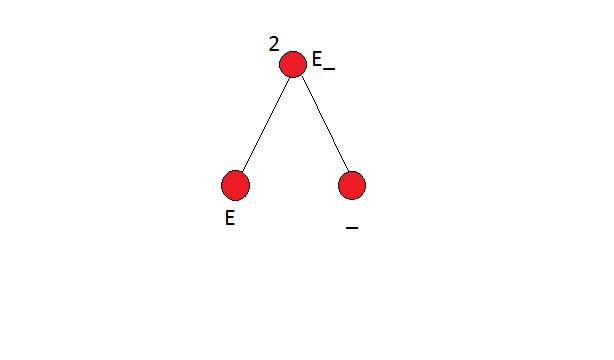
\includegraphics[scale=0.6]{1}
\end{frame}


\begin{frame}{Graphical Overview Of Huffman Coding}
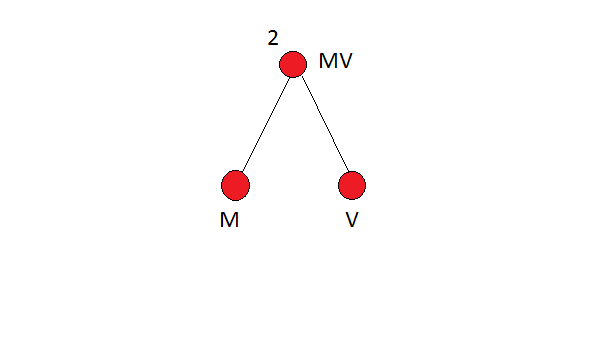
\includegraphics[scale=0.6]{2}
\end{frame}


\begin{frame}{Graphical Overview Of Huffman Coding}
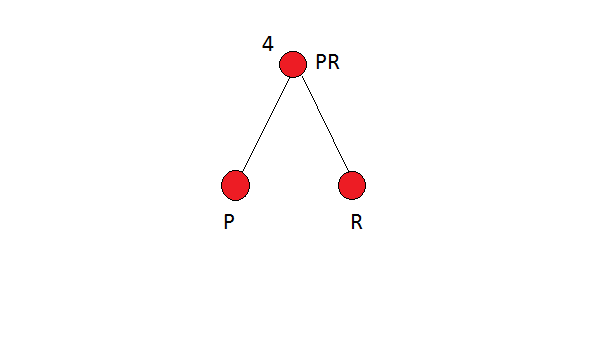
\includegraphics[scale=0.6]{3}
\end{frame}

\begin{frame}{Graphical Overview Of Huffman Coding}
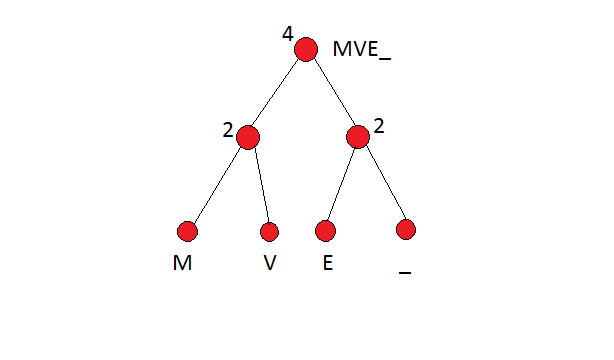
\includegraphics[scale=0.6]{4}
\end{frame}

\begin{frame}{Graphical Overview Of Huffman Coding}
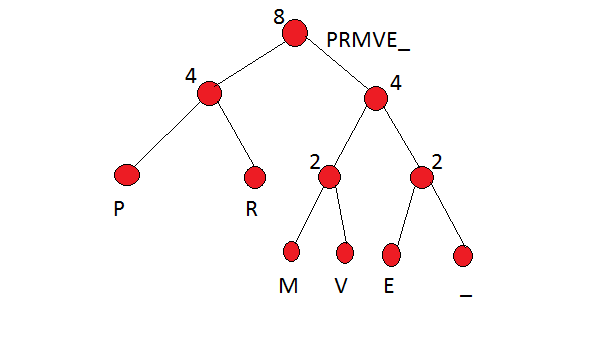
\includegraphics[scale=0.6]{5}
\end{frame}

\begin{frame}{Graphical Overview Of Huffman Coding}
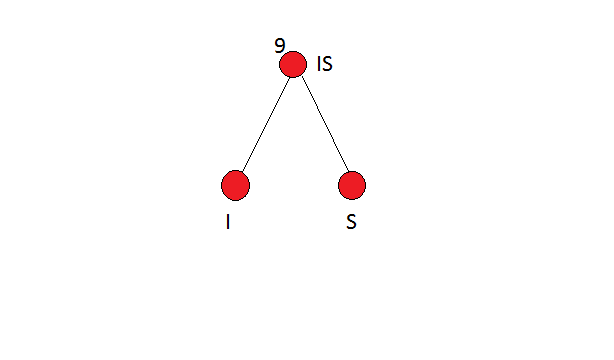
\includegraphics[scale=0.6]{6}
\end{frame}


\begin{frame}{Graphical Overview Of Huffman Coding}
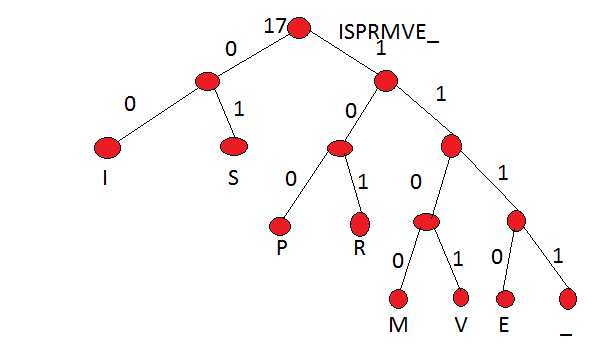
\includegraphics[scale=0.6]{7}
\end{frame}



\begin{frame} {Finally .... }

	

	\pause
     
     \begin{table}[bt]
	\begin{tabular}{|l|c|c|c|c|c|c|c|} \hline 
	\textbf{I} & \textbf{S} & \textbf{P} & \textbf{R} & \textbf{M} & \textbf{V} & \textbf{E} &\textbf{""} \\ \hline
	
	\textbf{00} & \textbf{01} & \textbf{100} & \textbf{101} & \textbf{1100} & \textbf{1101} & \textbf{1110} &\textbf{1111} \\ \hline
	\end{tabular}
\end{table}	
	

\end{frame}


\begin{frame}
      {\color{red}\textbf{After Huffman Coding Tree}}
	  \pause
	  
	 Number of bits= 5$*$2$+$4$*$2$+$2$*$3$+$2$*$3$+$4$*$1$+$4$*$1$+$4$*$1$+$4$*$1=46\\ 	  
	 
	 
	 \pause
	 
	 \textbf{\color{blue} Improvement:} 66.2\%  
	        
\end{frame}


\begin{frame} {Complexity}
	\begin{itemize}
		\item time complexity is {\color{orange}nlogn}
		\item can be improved by using 	{\color{orange}Van Embde Boss}
	\end{itemize}
\end{frame}
\begin{frame} {Usefullness}
\begin{itemize}
	\pause
	\item Easy To decode
	\pause
	\item Prefix free code
	\pause
	\item The tree generated by Huffman Code is a Full Binary Tree 
\end{itemize}
\end{frame}


\begin{frame} {Full Binary Tree}
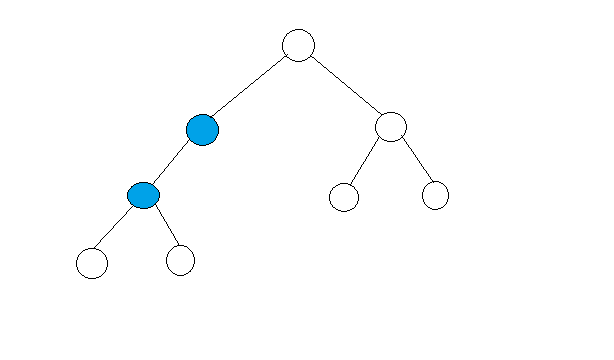
\includegraphics[scale=0.5]{full}
\end{frame}


\begin{frame}
		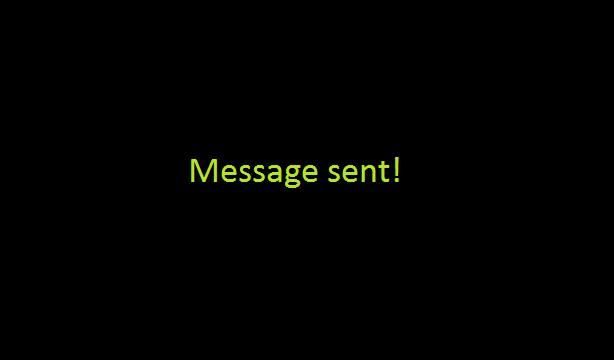
\includegraphics[scale=0.6]{sent}
\end{frame}

\begin{frame} {Resources}
\begin{thebibliography}
\bibitem Introduction To Algorithms by Thomas H. Cormen , Charles E. Leiserson , Ronald L.Rivest, Clifford Stein.
\end{thebibliography} 
\end{frame}



\end{document}



